253. \begin{figure}[ht!]
\center{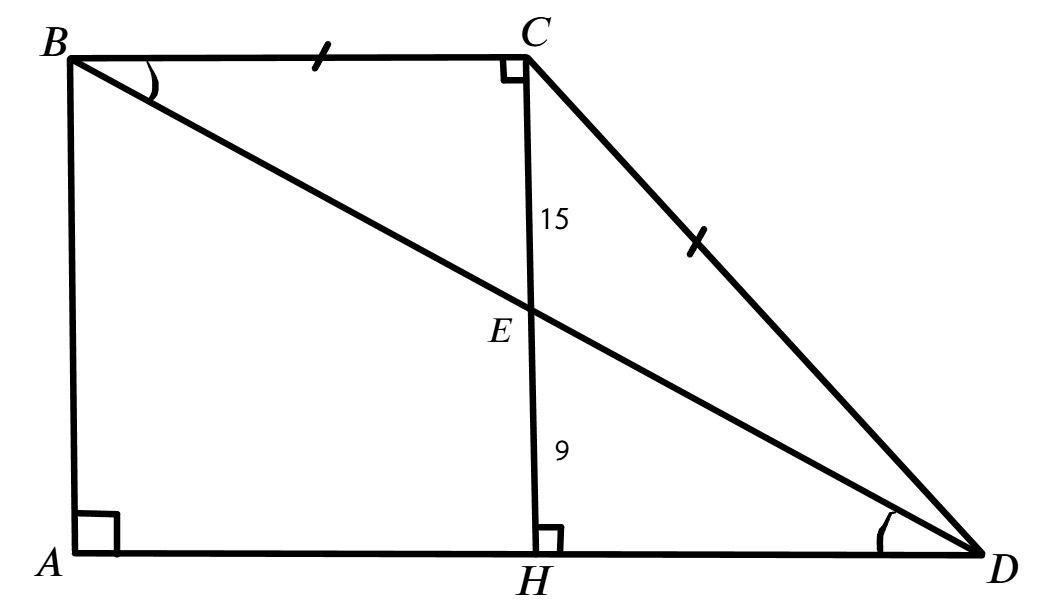
\includegraphics[scale=0.35]{g8-248.png}}
\end{figure}\\
Треугольники $BEC$ и $HED$ подобны по двум углам ($\angle EHD=\angle EBC$ и $\angle EDH=\angle EBC$ как накрест лежащие), поэтому $\cfrac{HD}{BC}=\cfrac{EH}{EC}=\cfrac{9}{15}=\cfrac{3}{5}.$ Тогда если $BC=CD=x,$ то по теореме Пифагора для треугольника $CDH$ получим равенство: $x^2=\cfrac{9}{25}x^2+24^2,\ \cfrac{16}{25}x^2=576,\ x^2=36\cdot25,\ x=6\cdot5=30$см и $HD=\cfrac{3}{5}\cdot30=18$ см. Тогда $AD=HD+BC=18+30=48$см и $S_{ABCD}=\cfrac{1}{2}\cdot24\cdot(30+48)=936\text{ см}^2.$
\end{document} 